\documentclass[xcolor=svgnames,handout]{beamer}

\usepackage[utf8]    {inputenc}
\usepackage[T1]      {fontenc}
\usepackage[english] {babel}
\usepackage{media9}
\usepackage{tikz}

\usepackage{amsmath,amsfonts,graphicx}
\usepackage{beamerleanprogress}


\title
  [Identificarea bolilor cardice cu re\c{t}ele neuronale\hspace{2em}]
  {Identificarea bolilor cardice cu re\c{t}ele neuronale}

\author
  [Lungu Daniel]
  {Coordonator \c{s}tiin\c{t}ific \quad Conf. Dr. Alexe Bogdan
  \\
  Absolvent\quad Lungu Daniel}

\date
  {Iunie, 2017}

\institute
  {Universitatea Bucure\c{t}i
  \\ Facultatea de Matematic\u{a} \c{s}i Informatic\u{a}
  \\ Specializarea Calculatoare \c{s}i Tehnologia Informa\c{t}iei}


\begin{document}

\maketitle

\section
  {Problema abordat\u{a} \^{i}n lucrare}

\begin{frame}
  {Problema abordat\u{a} \^{i}n lucrare}


\begin{itemize}
\item Ciclul s\^{a}ngelui prin inim\u{a} :
\begin{figure}[t]
    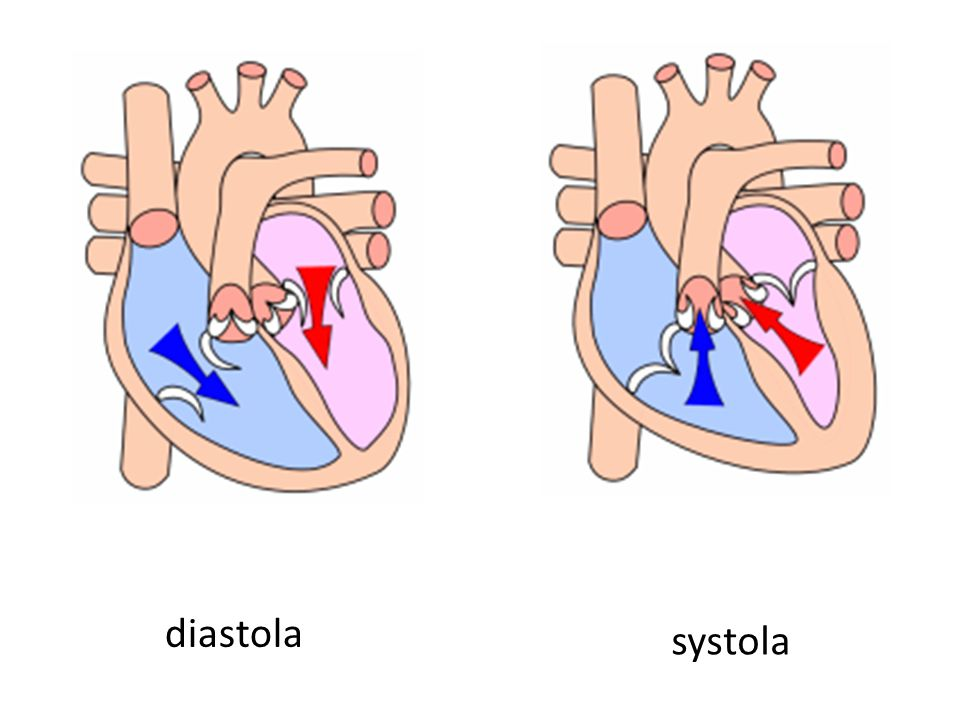
\includegraphics[width=7cm]{diastola+systola.jpg}
    \centering
\end{figure}
\item Diastol\u{a} : volumul maxim de s\^{a}nge prin inim\u{a}
\item Sistol\u{a} : volumul minim de s\^{a}nge prin inim\u{a}
 \end{itemize}
\end{frame}


\begin{frame}
  {Frac\c{t}ia de ejec\c{t}ie}

  \begin{itemize}
  \item Ecua\c{t}ie :
    \begin{equation*}
      E_{j} = 100 \frac{V_D - V_S}{V_D}
    \end{equation*}
    
  \item $V_D$ : volumul de s\^{a}nge la diastol\u{a}
  \item $V_S$ : volumul de s\^{a}nge la sistol\u{a}
  \item $E_j \geq $  75\% : hiperdinamic
  \item $E_j < 75 \% $ \c{s}i $E_j \geq $  55\% : normal
  \item $E_j < 55 \% $ \c{s}i $E_j \geq $  45\% : u\c{s}or anormal\u{a}
  \item $E_j < 45 \% $ \c{s}i $E_j \geq $  35\% : moderat anormal\u{a}
  \item $E_j < $  35\% : sever anormal\u{a}
  
  \end{itemize}
\end{frame}

\section
  {Datele folosite}

\begin{frame}
  {Datele folosite}

\begin{itemize}
\item Institutul Na\c{t}ional pentru Pl\u{a}m\^{a}ni, Inim\u{a} \c{s}i S\^{a}nge din America
  \begin{center}
    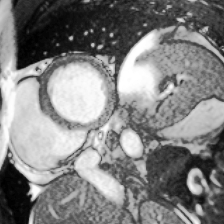
\includegraphics[width=50]{1.png}
    \hspace{0.15cm}
    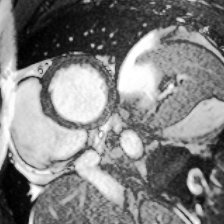
\includegraphics[width=50]{3.png}
    \hspace{0.15cm}
    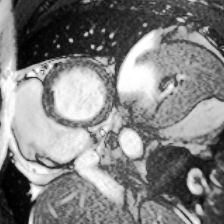
\includegraphics[width=50]{5.png}
    \hspace{0.15cm}
    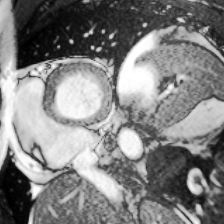
\includegraphics[width=50]{7.png}
    \hspace{0.15cm}
    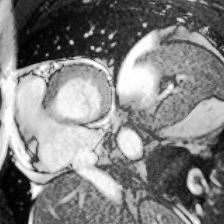
\includegraphics[width=50]{9.png}
  \end{center}
  
  \begin{center}
    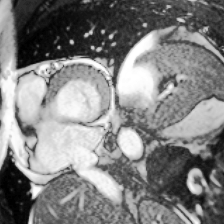
\includegraphics[width=50]{11.png}
    \hspace{0.15cm}
    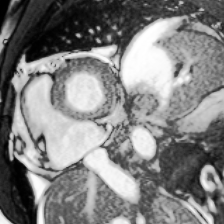
\includegraphics[width=50]{13.png}
    \hspace{0.15cm}
    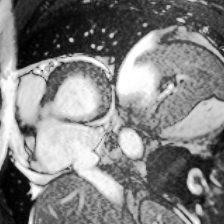
\includegraphics[width=50]{15.png}
    \hspace{0.15cm}
    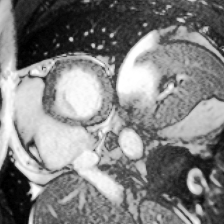
\includegraphics[width=50]{17.png}
    \hspace{0.15cm}
    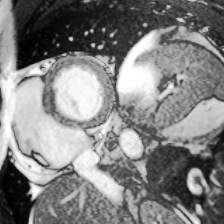
\includegraphics[width=50]{19.png}
  \end{center}
  
  \begin{center}
    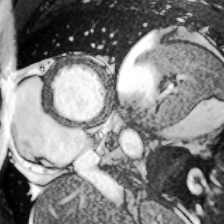
\includegraphics[width=50]{21.png}
    \hspace{0.15cm}
    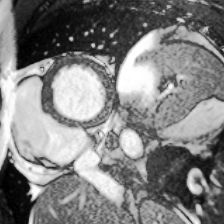
\includegraphics[width=50]{23.png}
    \hspace{0.15cm}
    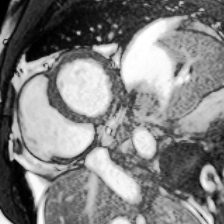
\includegraphics[width=50]{25.png}
    \hspace{0.15cm}
    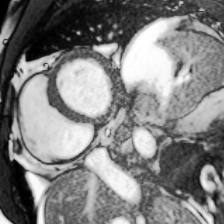
\includegraphics[width=50]{27.png}
    \hspace{0.15cm}
    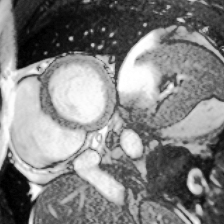
\includegraphics[width=50]{29.png}
  \end{center}
  \item Cadre : 30
  \item Segmente: 10 - 15
  \end{itemize}
\end{frame}

\begin{frame}
  {Datele folosite}
  
  \begin{itemize}
  \item Institutul Sunnybrook
      
    \begin{center}
        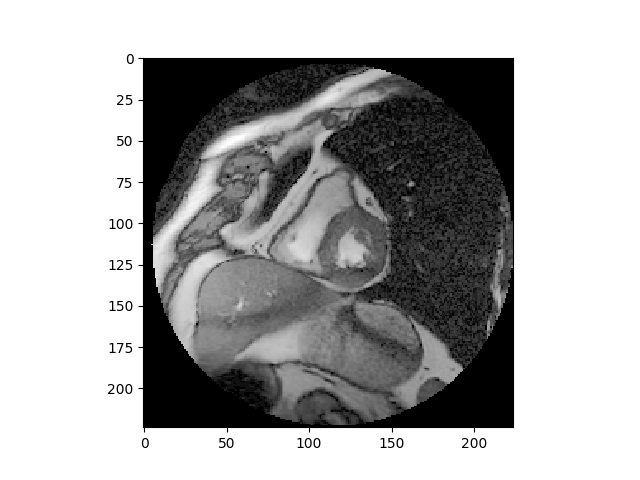
\includegraphics[width=120]{1_image.png}
        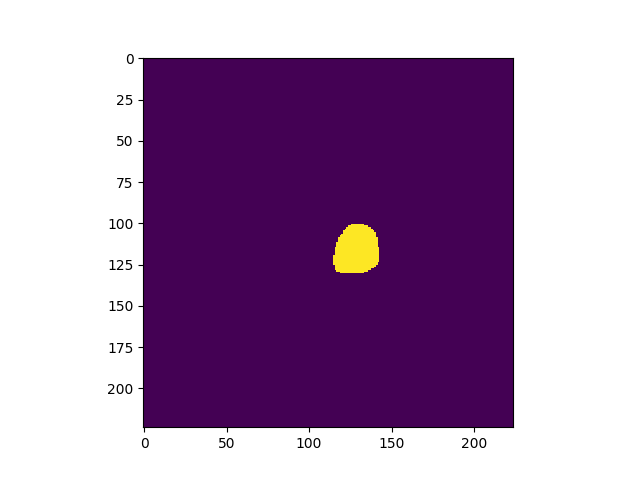
\includegraphics[width=120]{1_labels.png}  
    \end{center}
    
    \begin{center}
        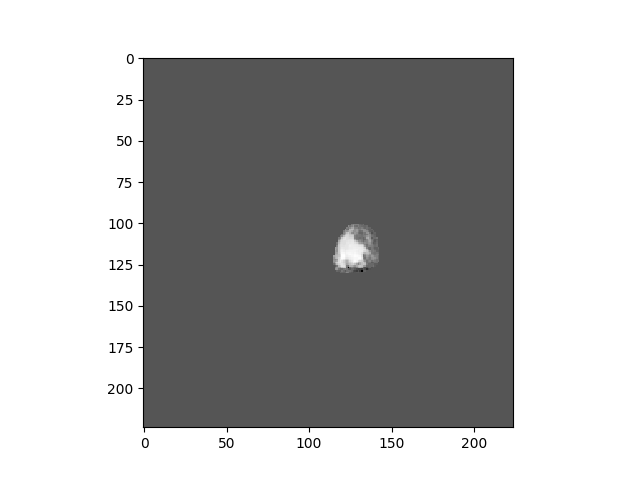
\includegraphics[width=120]{1_image_labels.png}
    \end{center}
 \item Format : DICOM
 \end{itemize}
\end{frame} 

\section
  {Solu\c{t}ia propus\u{a}}

\begin{frame}
  {Solu\c{t}ia propus\u{a}}
  
  \begin{itemize} 
    \item Preprocesarea datelor
    \item Re\c{t}ea neuronal\u{a} convolu\c{t}ional\u{a} pentru segmentarea ventriculului st\^{a}ng
    \item Calcularea volumului de s\^{a}nge la sistol\u{a} \c{s}i la diastol\u{a}
    \item Calibrarea datelor
    \item Calcularea frac\c{t}iei de ejec\c{t}ie 
  \end{itemize}
  \end{frame}
  
  \begin{frame}
  {Preprocesarea datelor}
  \begin{itemize}
    \item Convertirea din format DICOM \^{i}n format PNG
    \item Decuparea imagini
    \item Redimensionarea imagini la 256 x 256
    \item Aplicarea algoritmului CLAHE
    \vspace{0.5cm}
    \begin{center}
        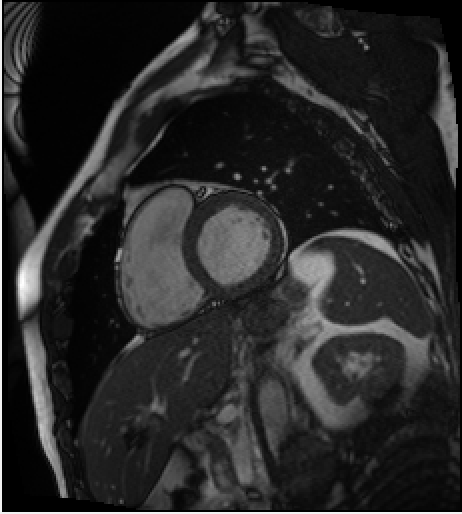
\includegraphics[width=110]{before.png}
        \hspace{2cm}
        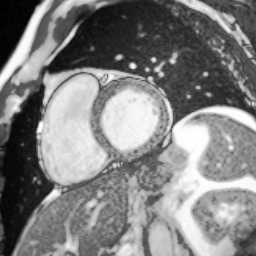
\includegraphics[width=110]{after.png}  
    \end{center}
  \end{itemize}
  \end{frame}
  
  \begin{frame}
    {Re\c{t}eauna neuronal\u{a} convolu\c{t}ional\u{a}}
    
    \begin{columns}[T]
    \begin{column}{.48\textwidth}
        \begin{itemize}
        \item Antrenare pe setul de date Sunnybrook
        \item Arhitecutr\u{a} asem\u{a}n\u{a}toare cu VGG
        \item Timp de antrenare : 5 ore
        \item Implementare : TensorFlow cu Python 3.5
        \item GPU : Nvidia Geforce Titan X
        \end{itemize}
    \end{column}%
    \hfill%
    \begin{column}{.48\textwidth}
    
    \begin{center}
        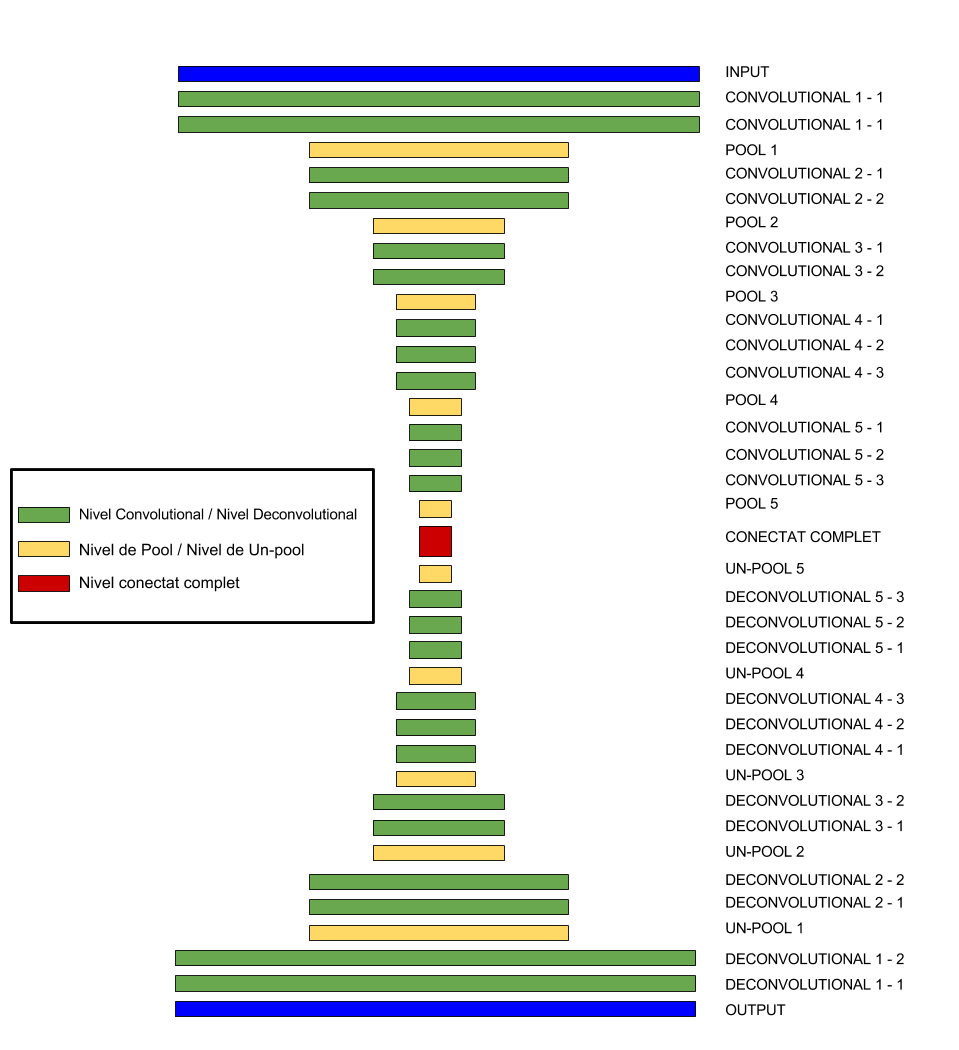
\includegraphics[width=170]{arhitectura_segmentor.png}  
    \end{center}
    \end{column}%
    \end{columns}
    
  \end{frame}
  
  \begin{frame}
    {Re\c{t}eauna neuronal\u{a} convolu\c{t}ional\u{a}}
  \begin{itemize}
    \item Rezultat:
       
    \begin{center}
        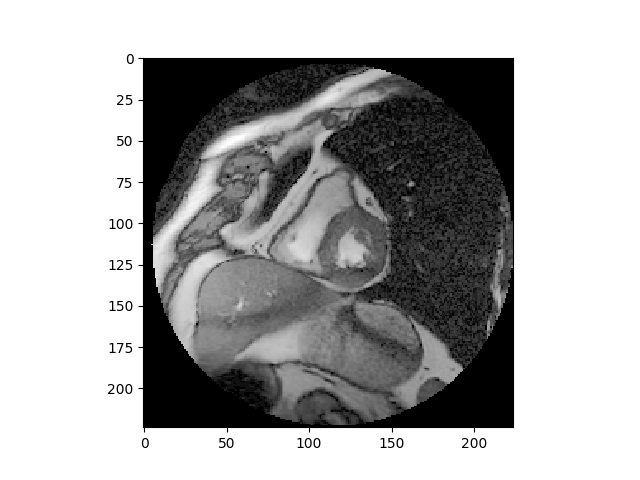
\includegraphics[width=110]{1_image.png}
        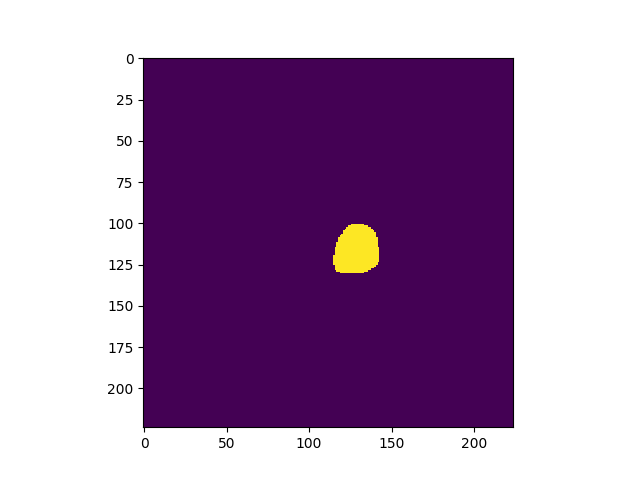
\includegraphics[width=110]{1_labels.png}
        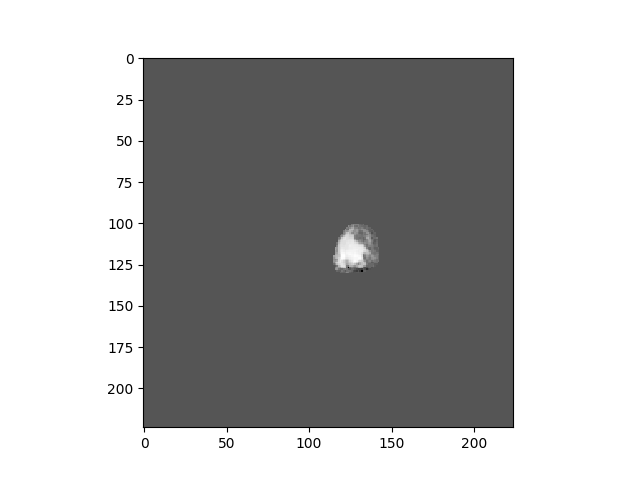
\includegraphics[width=110]{1_image_labels.png}
    \end{center}
    
    \begin{center}
        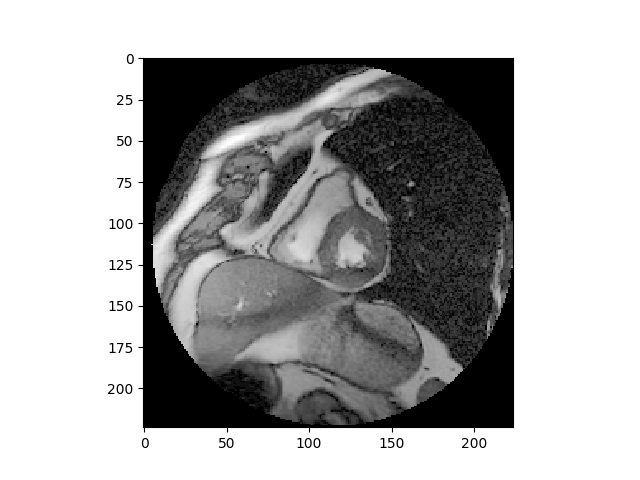
\includegraphics[width=110]{1_image.png}
        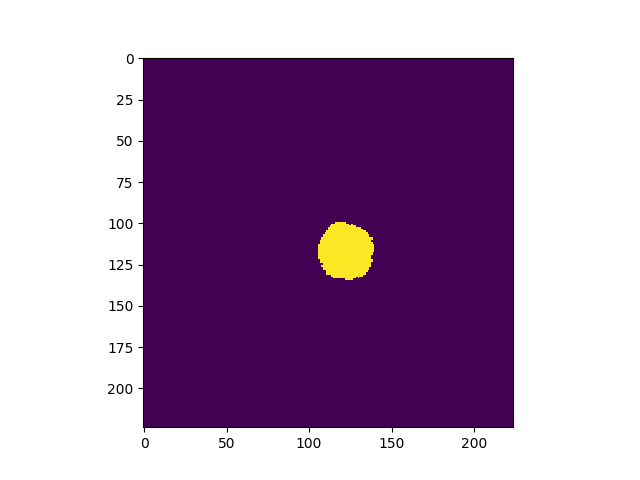
\includegraphics[width=110]{1_labels_predict.png}
        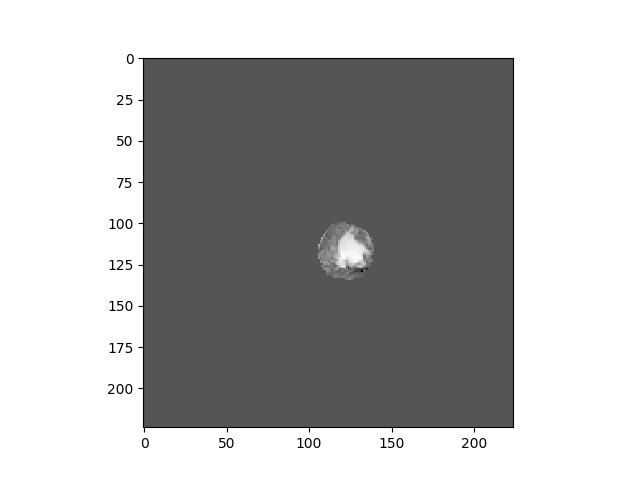
\includegraphics[width=110]{1_image_predict.png}
    \end{center}
  \end{itemize}
  \end{frame}
 
 \begin{frame}
    {Calcularea volumului de s\^{a}nge la sistol\u{a} \c{s}i la diastol\u{a}}
  \begin{itemize}
    \item Determinarea cadrului care apar\c{t}ine sistolei
    \item Determinarea cadrului care apar\c{t}ine diastolei
    \item Ecua\c{t}ie :
    
    \begin{equation*}
    V = \frac{1}{1000} \sum_i \Delta_i \frac{f_i + \sqrt{f_i * f_{i+1}} + f_{i+1}}{3}
    \end{equation*}
    \item $\Delta_i$ : distan\c{t}a dintre segmente
    \item V : volumul de s\^{a}nge
    \item $f_i$ : segmentul de la pozi\c{t}ia i
  \end{itemize}
  \end{frame}
    
    \begin{frame}
    {Calibrarea datelor \c{s}i calcularea frac\c{t}iei de ejec\c{t}ie}
    \begin{itemize}
        \item Calibrarea datelor : folosirea algoritmului Gradient Bootstrap Regresion pentru prezicerea volumului de s\^{a}nge
        \item Calcularea frac\c{t}iei de ejec\c{t}ie :
            \begin{equation*}
      E_{j} = 100 \frac{V_D - V_S}{V_D}
    \end{equation*}        
    \end{itemize}
  \end{frame}
    
    \section
  {Rezultate}
    
    \begin{frame}
  {Rezultate}
  
    \begin{center}
 \begin{tabular}{|p{0.3cm}|p{1.1cm}|p{1.1cm}|p{1.1cm}|p{1.1cm}|p{2cm}|p{2cm}|} 
 \hline
 Nr. & Diastola real\u{a} & Diastola prezis\u{a} & Sistola real\u{a} & Sistola prezis\u{a} & Frac\c{t}ia de ejec\c{t}ie pentru valorile reale & Frac\c{t}ia de ejec\c{t}ie pentru valorile prezise  \\ [0.5ex] 
 \hline\hline
 1 &  158.0 & 158.7 & 76.0 & 63.61 & 51,8\% & 59,9\% \\
 \hline
 2 &  44.2 & 35.69 & 15.6 & 12.94 & 64,7\% & 63,7\% \\ 
 \hline
 3 &  129.7 & 128.44 & 83.2 & 38.6 & 35,8\% & 69,9\% \\
 \hline
 4 &  121.1 & 126.34 & 39.2 & 53.79 & 67,3\% & 57,4\% \\
 \hline
 5 &  127.4 & 145.78 & 57.8 & 57.99 & 54,63\% & 60,2\% \\
 \hline
 6 &  177.7 & 188.18 & 76.4 & 77.49 & 57\% & 58,8\% \\
 \hline
 7 &  277.6 & 186.16 & 133.5 & 74.88 & 51,9\% & 59,7\% \\
 \hline
 8 &  210.1 & 209.73 & 167.5 & 102.7 & 20,2\% & 51\% \\
 \hline
 9 &  230.1 & 193.51 & 91.4 & 91.53 & 60.2\% & 52,7\% \\
 \hline
 10 &  315.8 & 213.66 & 122.3 & 98.24 & 61,2\% & 54\% \\
 \hline
\end{tabular}
\end{center}
  
  \end{frame}
  
  
  \begin{frame}
  
  \begin{center}
\Huge Mul\c{t}umesc !
\end{center}
  
    
    
\end{frame}
    
\end{document}